\documentclass[11pt]{article}

\usepackage[margin=0.8in]{geometry}
\usepackage{amsmath}
\usepackage{graphicx}
\usepackage{parskip}
\usepackage{float}
\usepackage[font=small,labelfont=bf]{caption}
\usepackage[colorlinks=true,linkcolor=blue!55!black]{hyperref}

\graphicspath{{../stage_connectivity_report/figures/}}

\begin{document}
\section*{What triggered this}

The panel below reports the test-loss chord barrier (the one we've used so far) after selecting the
best overall alignment separately for every ordered stage pair.  At the early
checkpoints, aligning $A_{200}$ with $B_n$ gives a much smaller barrier than
aligning $A_n$ with $B_{200}$.  For example, at $n=0$ the means are $0.300$
and $0.699$, respectively; at $n=1$ they are $0.316$ and $0.589$.

\begin{figure}[H]
    \centering
    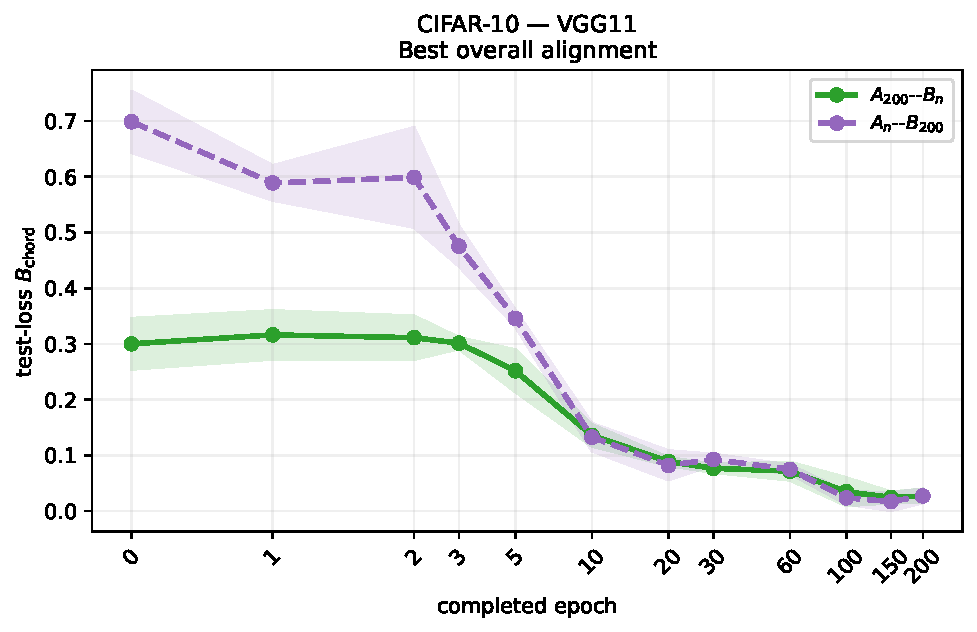
\includegraphics[width=0.67\linewidth]{vgg11_original_figure3_right_test_loss.pdf}
    \caption{Mean $\pm$ one standard deviation over three seed pairs.}
\end{figure}

This is not just an $A$--$B$ path traversed backwards.  The two comparisons
are $A_{200}$--$B_n$ and $A_n$--$B_{200}$, so they use different checkpoints.
They should nevertheless have the same distribution if the A/B roles and the
alignment procedure are exchangeable.

At $n=0,1,2,3$, both VGG11 directions selected Sinkhorn followed by scale
fine-tuning.  Across the full $12\times12$ ordered matrix, Sinkhorn+scale was
selected in 91 cells and almost always when $n$ was small (big difference in training stages between networks), compared with 53 cells for WM+scale (performing better when $n$ was big, indicating small difference in networks' training stages) . 

\clearpage
\section*{Fixed-method check: CIFAR-10 / VGG11}

To separate method selection from method behaviour, the next two plots keep
the method fixed.  ``Sinkhorn with scale'' here means a hard Sinkhorn permutation
followed by positive-scale fine-tuning.  The second method is WM+scale.

\begin{figure}[H]
    \centering
    \begin{minipage}[t]{0.49\linewidth}
        \centering
        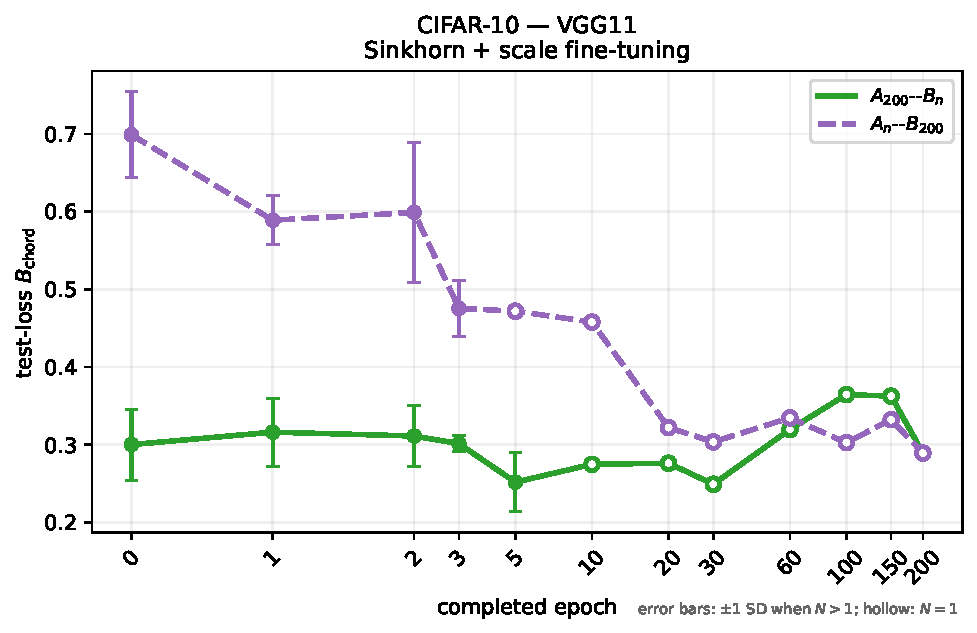
\includegraphics[width=\linewidth]{cifar10_vgg11_sinkhorn_scale_cross_stage_test_loss.pdf}
    \end{minipage}\hfill
    \begin{minipage}[t]{0.49\linewidth}
        \centering
        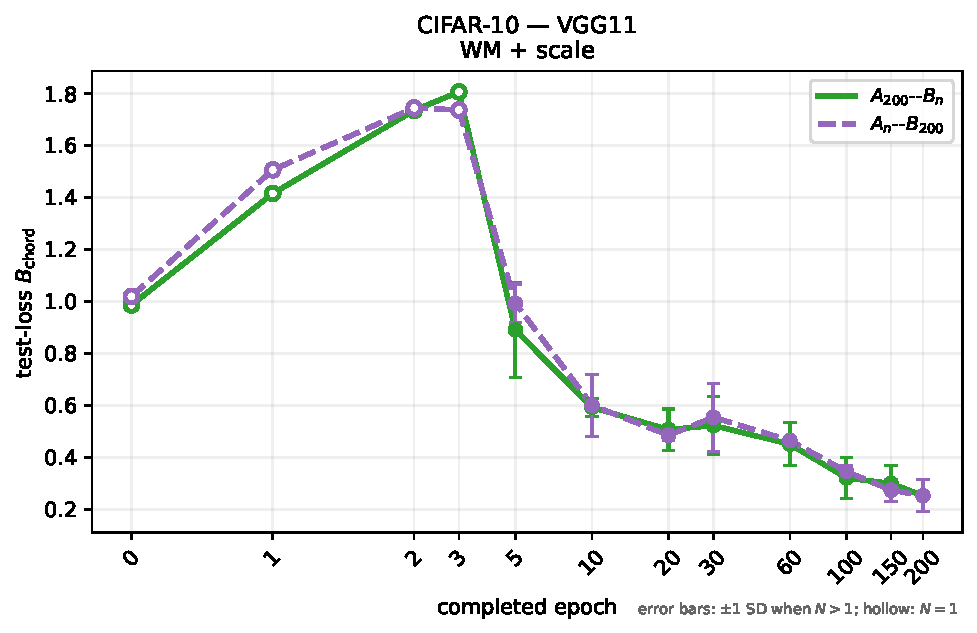
\includegraphics[width=\linewidth]{cifar10_vgg11_wm_cross_stage_test_loss.pdf}
    \end{minipage}
    \caption{VGG11 fixed-method diagnostic.  Sinkhorn+scale is strongly
    directional for early/final pairs.  WM+scale is much closer to symmetric,
    especially at the earliest stages.  Error bars show $\pm1$ SD wherever
    multiple seed pairs were evaluated; hollow points have only one pair.}
\end{figure}

\section*{Short interpretation}

The permutation-matching part of WM+scale approximately solves
\[
    P^\star=\arg\min_P \|\theta_A-P\theta_B\|_2^2.
\]
For an exact solution on the same endpoint pair, swapping A and B simply uses
the inverse permutation, so the objective itself is direction-independent.
The implementation is greedy and the plotted stage slices are not literal
reversals, so small WM+scale differences are still possible; however, as seen
in the plot, the directional variation is very small.

The Sinkhorn implementation is operationally directional.  One endpoint is
kept fixed, while a permutation (and then scales) is optimized only for the
other endpoint using interpolation loss.  The transform starts at identity;
the relevant difference is which checkpoint is fixed and which checkpoint is
allowed to move.  Empirically, in the early/final comparison,

\begin{center}
    early model $\longrightarrow$ fixed final model
\end{center}

works substantially better than

\begin{center}
    final model $\longrightarrow$ fixed early model.
\end{center}

I observed similar results for the MLP trained on Fashion-MNIST.

\end{document}
